\chapter{Testing}

Il \textbf{testing} è un sottoinsieme di un ambito più generale: la \textbf{\textit{verifica}}.
Questa può essere \textit{soggettiva} o \textit{oggettiva}, e si può concentrare su qualità interne o esterne. Il risultato del processo di testing non è una risposta binaria (SI o NO), ma l'individuazione di difetti con diversi \textit{livelli di severità}.
\\
\\
Gli \textit{approcci alla verifica} sono di tipo:
\begin{itemize}
    \item \textbf{Dinamico} (testing) in cui si valuta il comportamento del software in esecuzione
    \item \textbf{Statico} in cui si analizzano le proprietà del prodotto software
\end{itemize}

\paragraph{Testing} Consiste nell'ottenere \textbf{campioni di comportamento} sottoponendo il programma a particolari \textit{test-case}: configurazioni di input e casistiche. \textit{Manca di continuità} poiché non è definibile un test in grado di garantire che il comportamento del sistema sia corretto in ogni situazione. Idealmente un test dovrebbe essere \textbf{ripetibile} ovvero presentare stessi risultati sotto le stesse condizioni, caratteristica influenzata da: ambiente esterno, task con esiti non deterministici (es. generazione di numeri pseudo-random).

\paragraph{Dijkstra (1987)} “L'obiettivo del testing è individuare la presenza di bug nel sistema ed isolarli attraverso l'applicazione di principi sistematici e metodi accurati, di modo da facilitare la loro correzione” (\textit{debugging})

\paragraph{Formalmente} Dati $D$ insieme dei possibili input ed $R$ insieme dei possibili output, un programma $P$ è definito come:
\begin{center}
    $P : D \rightarrow R$
\end{center}
Funzione \textbf{parziale} poiché potrebbero esistere elementi di $D$ non corrispondenti ad alcun elemento in $R$ (funzione non definita).

\paragraph{Nota} Il testing del software è afflitto dal \textbf{problema dell'oracolo} (entità responsabile di esaminare i risultati dei test, stabilendo se siano accettabili o meno). Spesso far valutare ogni risultato da un operatore umano risulta essere lento e inefficiente: è necessario “automatizzare” l'oracolo. La progettazione di un oracolo automatico è un processo complesso e privo di una soluzione universalmente valida:
\begin{itemize}
    \item lo sviluppo D-by-C favorisce l'analisi automatica del testing; 
    \item la presenza di specifiche informali o di molti fattori esterni rende spesso necessario un oracolo umano.
\end{itemize}
Inoltre, il testing non dovrebbe limitarsi a verificare le funzionalità di un sistema software, ma dovrebbe anche affrontare:
\begin{itemize}
\item \textit{Overload}: risposta del sistema a carichi di lavoro eccessivi;
\item Robustezza e regressione del sistema;
\item Concorrenza (che introduce effetti non deterministici);
\item Diverse configurazioni temporali (solo nei sistemi real time);
\end{itemize}

\section{Correttezza}

La correttezza del programma è descritta dal sottoinsieme:
\begin{center}
$O \subseteq D \times R$    
\end{center}
Preso $d \in D$, un \textbf{output $P(d)$ è corretto} se la coppia $\langle d, P(d) \rangle$ è ammissibile (appartiene ad $O$). Un \textbf{programma $P$ è corretto} se ogni suo output è corretto (verificabile solo per $D$ finito). Un output si dice \textbf{fallimento} se è errato per l'input $d$ o se $P(d)$ non è definito. Un \textbf{errore} è la causa di un fallimento, al suo verificarsi il programma entra in uno stato intermedio incorretto: \textbf{fault}.

\paragraph{Test Case} Definito come $t \in D$, ha successo SSE $P(t)$ è corretto.

\paragraph{Test Set} Definito come $T \subseteq D$, ha successo SSE $P(t)$ è corretto $\forall t \in T$. Nel caso in cui il programma $P$ è scorretto, un test set si dice \textbf{ideale} se $\exists t \in T$ t.c. $P(t)$ non è corretto.

\section{Criteri di testing}

Un \textbf{criterio} è una regola per definire dei sottoinsiemi finiti di $D$ (test set).
Sia $2^D$ l'insieme di tutti i possibili sottoinsiemi di $D$, $C$ è un insieme tale che:
\begin{center}
    $C \subseteq 2^D$ (finito)
\end{center}
Un \textbf{test set $T$ soddisfa} un criterio $C$ se:
\begin{center}
    $T \in C$    
\end{center}

\paragraph{Esempio} Sia $D$ il dominio dei numeri interi, definiamo il seguente criterio:
\begin{center}
    $C = \{x_1, x_2, ..., x_n\} | n \ge 3 \cap \exists i, j, k | x_i < 0, x_j = 0, x_k > 0$    
\end{center}
Il criterio richiede un test set tale per cui esistano almeno 3 numeri interi: uno positivo, uno negativo ed uno pari a zero.
\begin{center}
    $T_1 = \{-5, 0, 12\}$ soddisfa $C$    
\end{center}
\begin{center}
    $T_2 = \{9, 0, 18\}$ NON soddisfa $C$    
\end{center}

\subsection{Proprietà}

\paragraph{Consistenza} Dato un criterio $C$, comunque si prendano $T_1, T_2 \in C$, $T_1$ ha successo SSE anche $T_2$ ha successo. Ergo: tutti i test set che soddisfano $C$ sono equivalenti e danno lo stesso risultato.

\paragraph{Completezza} Un criterio $C$ è detto \textbf{completo} se, posto il programma $P$ non corretto, esiste almeno un test set $T \in C$ che non ha successo.
\\
\\
Nella pratica non è possibile definire un algoritmo che stabilisca se un criterio sia consistente e completo. Ciò non significa che i test set possano essere scelti senza criterio ed in modo casuale (sarebbe inadeguato).

\paragraph{Finezza} Un criterio $C_1$ si dice \textbf{più fine} di un criterio $C_2$ se investiga più casi, deve valere che:
\begin{center}
    $\forall P, \forall T$ che soddisfa $C1$, $\exists T^I \subset T$, con $T^I \in C_2$
\end{center}
Il testing, guidato dall'\textit{esperienza empirica}, è mirato alla definizione di \textbf{test set significativi} che hanno buone probabilità di rilevare la presenza di errori.

\paragraph{Criterio della copertura completa} Criterio empirico che prevede due fasi. Nella prima fase si divide il dominio $D$ in una serie di \textit{sottodomini} $Di$
\begin{center}
    $\{D_1, D_2, … ,D_n\}\ |\ D = D_1 \cup D_2\ \cup\ ... \cup\ D_n$
\end{center}
che rispettano le proprietà: riflessiva, simmetrica e transitiva.
Se i sottodomini sono \textit{disgiunti} ($D_i \cap D_j = \emptyset$) si dice che costituiscono una \textbf{partizione} di $D$. In una seconda fase si crea un test set selezionando un elemento per ogni sottodominio $D_i$, se non formano una partizione si possono scegliere gli elementi in comune per \textit{minimizzare} la dimensione del test set.
\\
\\
I criteri di testing partizionano il dominio di input $D$ in \textbf{classi di equivalenza}, la maggior parte degli errori in un software tende a concentrarsi nelle “\textit{zone di confine}” fra le classi. Un test set dovrebbe prediligere le condizioni di confine (\textit{boundary}) rispetto alle condizioni interne.

\section{Strategie di testing}

Il testing di componenti software può seguire due strategie complementari (idealmente andrebbero applicate entrambe).

\subsection{White Box - Strutturale}

Il criterio di partizione per derivare il test set si basa sul codice del componente (trasparente, visibile), deve testare ogni parte significativa del codice ("copertura strutturale") altrimenti è inadeguato e si concentra sul flusso di controllo del codice verificando esattamente ciò che il componente fa.

\subsubsection{Tipologie}

\paragraph{Statement Coverage} Si seleziona un test set tale da far eseguire almeno una volta ogni istruzione elementare del componente; Il limite del criterio è che provare ogni istruzione del codice non significa assicurarsi di esplorare ogni possibile flusso di esecuzione; 
   
\paragraph{Edge Coverage} Si seleziona un test set tale da esplorare almeno una volta ogni possibile flusso di esecuzione del componente. Richiede la costruzione preliminare del “grafo di controllo” del codice: 
\begin{itemize}
	   \item gli archi (orientati) rappresentano un'istruzione; 
	   \item il nodo d'uscita dell'arco è la condizione di partenza dell'istruzione;
	   \item il nodo d'ingresso è la condizione d'arrivo dell'istruzione. 
\end{itemize}
Il criterio prevede che ogni ramo del grafo di controllo del codice sia preso in considerazione almeno una volta. Il limite del criterio è che pur esplorando ogni ramo del flusso, non coglie i differenti motivi che possono portare a seguire un ramo se la condizione d'ingresso è composta; 
   
\paragraph{Condition Coverage} Si seleziona un test set tale da esplorare almeno una volta ogni possibile flusso di esecuzione del componente e di valutare in maniera indipendente almeno una volta ogni valore costituente di condizioni composte. Il limite del criterio è che alle volte non basta ispezionare ogni istruzione del codice e tutti i flussi di controllo per rilevare l'errore: alcune istruzioni possono comportare errore per determinati input e non per altri; 
   
\paragraph{Path Coverage} Si seleziona un test set tale da esplorare tutti i possibili percorsi dal nodo iniziale al nodo finale del grafo di controllo. Il limite è che il numero di percorsi potrebbe essere troppo elevato o addirittura infinito (cicli), rendendo il criterio inapplicabile (\textit{path explosion});

\begin{figure}[h!]
    \centering
    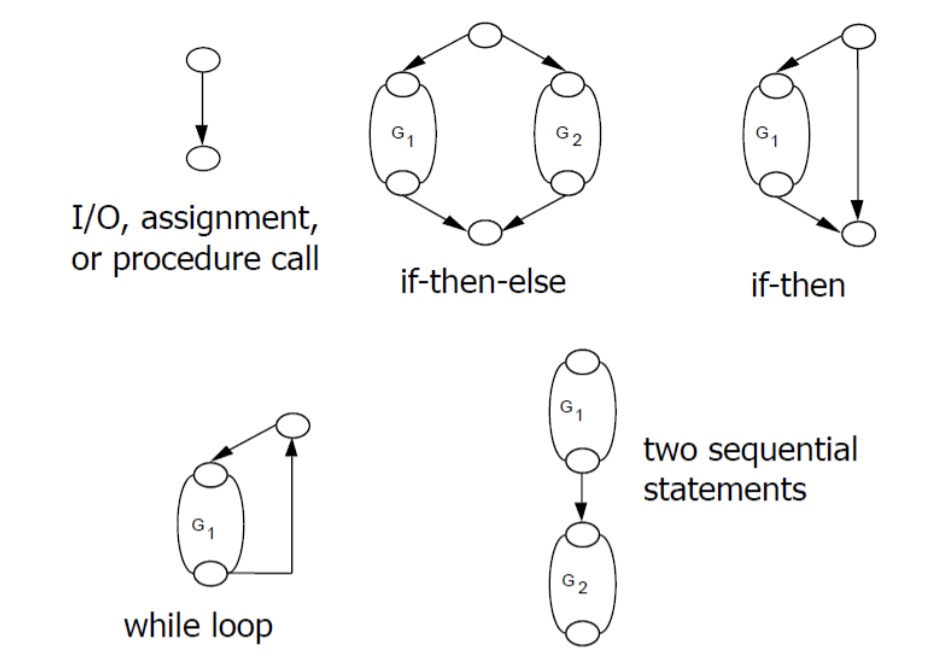
\includegraphics[width=0.75\linewidth]{assets/wb-control-graph.png}
    \caption{Regole di costruzione del grafo di controllo}
    \label{fig:wb-graph}
\end{figure}

\subsubsection{Limiti}
Potrebbe essere infattibile coprire l'intera struttura del codice, riducendo la percentuale di adeguatezza del test. Inoltre, il personale adibito ai test deve avere una buona conoscenza del programma e il test dipende strettamente dall'implementazione:
\begin{itemize}
    \item se l'implementazione cambia è necessario modificare anche il test; 
    \item tutti gli elementi della specifica che non sono esplicitamente implementati nel codice vengono ignorati. 
\end{itemize}

\subsection{Black Box - Funzionale}

Il criterio di partizione per derivare il test set si basa sulla specifica del componente, astraendo dal codice. Piuttosto si verifica ciò che il componente si propone di fare. È riusabile per più programmi perché NON DIPENDE DALL'IMPLEMENTAZIONE MA SI BASA SULLA SPECIFICA DEL MODULO. Si cerca di derivare un test set significativo a partire dalla specifica del componente, cercando di:
\begin{itemize}
    \item coprire tutte le possibili situazioni di funzionamento
    \item trovare dei \textit{controesempi} (situazioni in cui il componente potrebbe non funzionare). 
\end{itemize}

\subsubsection{Tipologie}

\paragraph{Testing derivato da pre-condizioni e post-condizioni logiche del componente} Adatto a componenti DBC

\paragraph{Testing derivato dal linguaggio degli input attesi dal programma} Si cerca di avere una copertura totale della sintassi (ogni regola grammaticale deve essere esercitata almeno una volta). È indicato per testare sistemi software come compilatori o interpreti. Essendo la sintassi di un linguaggio un oggetto formale, i test set si prestano ad essere generati automaticamente.

\paragraph{Testing basato su tabella delle decisioni} Rappresentazione tabulare dei possibili input in relazione alle diverse condizioni in cui il sistema può trovarsi, la cella indica:
\begin{itemize}
    \item ($true$) determina - condizione soddisfatta;
	\item ($false$) non determina - condizione non soddisfatta;
\end{itemize}
La tabella mostra tutte le possibili combinazioni di input, aiutando i progettisti a derivare sistematicamente un test set;

\paragraph{Testing basato su grafi causa-effetto} Rappresenta i diversi effetti di possibili combinazioni di input, da cui derivare sistematicamente il test set. Nel grafo sono presenti dei nodi:
\begin{itemize}
    \item AND (due o più combinazioni si verificano contemporaneamente) 
	\item OR (si verifica almeno una di due o più combinazioni).
\end{itemize}
Il criterio di copertura prevede di testare tutte le possibili combinazioni di input, il numero di combinazioni da testare si può ridurre partendo dagli output e procedendo a ritroso:
\begin{itemize}
	\item se si incontra un nodo OR con output $true$ è sufficiente che solo una delle combinazioni in ingresso sia $true$ 
	\item se si incontra un nodo AND con output $false$ è sufficiente che solo una delle combinazioni in ingresso sia $false$
\end{itemize}

\section{Fasi di testing}

\subsection{Test dei singoli moduli}

La difficoltà risiede nelle possibili dipendenze da altri moduli, si deve ricorrere a delle componenti software che “simulano” gli elementi con cui il modulo si troverà ad interagire:
\begin{itemize}
    \item \textbf{driver}: modulo che attiva il modulo testato; 
	\item \textbf{stub}: modulo che viene usato dal modulo testato;
\end{itemize}

\begin{figure}[h!]
    \centering
    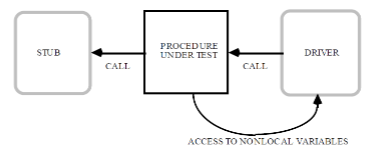
\includegraphics[width=0.75\linewidth]{assets/driver-stub.png}
    \label{fig:driver-stub}
\end{figure}

\subsection{Test di integrazione}
Si testano insiemi di moduli, ottenuti secondo due strategie.

\paragraph{Big Bang} L'insieme si ottiene (e viene testato) solo dopo aver sviluppato e testato singolarmente ogni modulo.

\paragraph{Incrementale} Non appena un modulo viene sviluppato e testato, lo si integra nell'insieme e si procede al test complessivo tramite approccio:
\begin{itemize}
    \item \textbf{bottom-up}: si usano \textit{driver}
    \item \textbf{top-down}: si usano \textit{stub}
\end{itemize}

\subsection{Test di sistema} Si testa il sistema complessivo (\textbf{\textit{Alpha Test}}).

\subsection{Test di accettazione} Valutazione da parte dei clienti di una versione rilasciata del sistema (\textbf{\textit{Beta Test}}).

\newpage
\paragraph{Testing con POO}

La \textit{Programmazione Orientata agli Oggetti} introduce nuovi aspetti (ereditarietà, polimorfismo, dynamic binding) di cui tenere conto nel testing. Una gerarchia di classi può essere testata tramite due strategie.

\paragraph{Appiattimento}  Si considera ogni classe concreta totalmente indipendente dalle altre.

\paragraph{Strategie ad-hoc} Traggono vantaggio dalla struttura gerarchica:
\begin{itemize}
	\item usare test che non devono essere ripetuti per ogni erede;
	\item usare test che devono essere eseguiti per una classe e tutti i successivi eredi;
	\item ripetere test con gli stessi input, verificando solo se l'output sia cambiato o meno;
	\item ripetere test aggiungendo parametri all'input e verificando che l'output cambi di conseguenza; 
\end{itemize}

\newpage